\documentclass[10pt, a4paper]{article}
\usepackage{algorithmic}
%\usepackage{savesym}
%\savesymbol{IF, algorithmic}
\usepackage[utf8]{inputenc}
\usepackage[spanish]{babel}
\usepackage[paper=a4paper, left=1.4cm, right=1.4cm, bottom=1.4cm, top=1.4cm]{geometry}
\usepackage{aed2-symb}
\usepackage{textcomp}
\usepackage[section, ruled]{algorithm}
\usepackage{hyperref}
\usepackage[pdftex]{graphicx}
\usepackage{epsfig}

\floatname{algorithm}{Algoritmo} % para que diga ``Algoritmo'' y no ``Algorithm''

\renewcommand{\algorithmiccomment}[1]{\ \ \ \textbf{//#1}} %para agregar comntarios en los algoritmos poner
% \COMMENT{ALAN ES GAY}
% \usepackage{algpseudocode}
% \usepackage{lineno}
\newenvironment{parr}
{\begin{list}{}%
         {\setlength{\leftmargin}{2em}}%
         \item[]%
}
{\end{list}}
\newcommand{\tab}{\hspace*{2em}}

\newcommand{\oper}[3]{\samepage\textsc{#1}(#2) $\rightarrow$ \textit{res} $\colon$ #3\\*}
\newcommand{\operL}[3]{\samepage\textsc{#1}(#2) $\rightarrow$ \textit{res} $\colon$ #3}
\newcommand{\operM}[2]{\samepage\textsc{#1}(#2)\\} %�sta es la operaci�n que no devuelve nada
\newcommand{\operMA}[2]{\samepage\textsc{#1}(#2)} %�sta es la operaci�n que no devuelve nada y para usar en el
%``caption'' del ``algorithm''
\newcommand{\vin}[2]{\textbf{in} \textit{#1}$\colon$#2}
\newcommand{\vinout}[2]{\textbf{in/out} \textit{#1}$\colon$#2}
\newcommand{\pre}[1]{\textbf{Pre} $\equiv$ \{#1\}\\*}
\newcommand{\post}[1]{\textbf{Post} $\equiv$ \{#1\}\\*}
\newcommand{\complej}[1]{\textbf{Complejidad:} #1\\*}
\newcommand{\desc}[1]{\textbf{Descripci\'on:} #1\\}
\newcommand{\alias}[1]{\textbf{Aliasing:} #1\\}

% \oper{nombre}{recibe}{devuelve}
% \vin{var}{tipo}
% \vinout{var}{tipo}
% \pre{}
% \post{}
% \complej{O()}
% \desc{txt}
% \alias{txt}

\newcommand{\eqobs}{$=_{obs}$}
\newcommand{\bigo}[1]{O$\big($#1$\big)$}
\newcommand{\NULL}{\textsc{Null} }
\newcommand{\aux}[3]{\samepage #1$\colon$ #2 $\rightarrow$ #3\\*}

\usepackage{hyperref}
\usepackage{color}
\usepackage{paralist}
\usepackage{multirow}
\usepackage{footnote}
\makesavenoteenv{tabular}
\usepackage{pdflscape}
\usepackage{enumitem}
\usepackage{amsmath}
\usepackage{caption}
\usepackage{subcaption}

\usepackage{lscape} 

%El siguiente paquete permite escribir la caratula facilmente
\usepackage{caratula}
\hypersetup{
  pdftitle={ Métodos Numéricos - TP1 },
  colorlinks,
  citecolor=black,
  filecolor=black,
  linkcolor=black,
  urlcolor=black 
}



\newlength{\AnchoEncabezados}\setlength{\AnchoEncabezados}{6em}
\newcommand{\EncabezadoInline}[2]{
    
    \setlength{\hangindent}{\tadAnchoEncabezados + \parindent}%
    
        \parbox{\AnchoEncabezados}{\textbf{#1}}#2%
}



\newcommand{\Encabezado}[2]{%
    \par\EncabezadoInline{#1}{#2}\par%
}

\newcommand{\funcion}[2]{\textbf{#1}{#2}\BlankLine}

\newcommand{\myFuncion}[3]{
	\begin{algorithm}[H][H]
	\dontprintsemicolon
	{\bf {#1}} {#2}\;
	\nocaptionofalgo
	\Indp
	{#3}
	\Indm
	\BlankLine
	\end{algorithm}
}
   
%Datos para la caratula
\materia{Métodos Numéricos}

\titulo{TP I - Métodos Numéricos}

%\fecha{DDDD dd de MMMM, AAAA}

\grupo{Grupo 2}

\integrante{Alejandro Dan\'os}{381/10}{adp007@msn.com}
\integrante{Franco}{}{}
\integrante{Fernando}{56/09}{yolibertino@gmail.com}
\integrante{Ana Sarri\'es}{144/02}{abarloventos@gmail.com}
\begin{document}

 %esto construye la caratula
 \maketitle
 \tableofcontents


\newpage

\section{Introducción Teórica}
%Contendrá una breve explicación de la base teórica que fundamenta los métodos involu-
%crados en el trabajo, junto con los métodos mismos. No deben incluirse demostraciones
%de propiedades ni teoremas, ejemplos innecesarios, ni definiciones elementales (como
%por ejemplo la de matriz simétrica). En vez de definiciones básicas es conveniente citar
%ejemplos de bibliografía adecuada. Una cita vale más que mil palabras.
%


\section{Desarrollo}
%Deben explicarse los métodos numéricos que utilizaron y su aplicación al problema
%concreto involucrado en el trabajo práctico. Se deben mencionar los pasos que si-
%guieron para implementar los algoritmos, las dificultades que fueron encontrando y la
%descripción de cómo las fueron resolviendo. Explicar también cómo fueron planteadas
%y realizadas las mediciones experimentales. Los ensayos fallidos, hipótesis y conjeturas
%equivocadas, experimentos y métodos malogrados deben figurar en esta sección, con
%una breve explicación de los motivos de estas fallas (en caso de ser conocidas).

Decidimos pensar al problema como si un sistema lineal de ecuaciones o, 
equivalentemente, buscar el vector x que cumpla $Ax=b$, siendo éstas las siguientes:
\begin{compactitem}
  \item Matriz A: es una matriz cuadrada con cantidad de filas y de columnas igual a $n \times m$ 
  	está dividida en 3 partes según las filas.  Sean i,j tal que $1 \leq i,j \leq (n \times m)$. \\
  	\begin{compactitem}
	  \item \textbf{Caso} $i \leq n$ \textbf{ó Caso} $(n \times m) - n < i$:
	    \[ A_{ij} = \left\{ \begin{array}{ll}
               1 & \mbox{si $i = j$};\\
	       0 & \mbox{si $i \neq j$}.\end{array} \right. \] 
          \item \textbf{Caso} $n < i \leq (n \times m) - n$:
	    \[ A_{ij} = \left\{ \begin{array}{ll}
               \frac{-2}{(\Delta r)^2} + \frac{1}{r \times \Delta r} - \frac{2}{r^2 \times (\Delta \theta)^2}& \mbox{si $i = j$};\\ \ \\
               \frac{1}{(\Delta r)^2} - \frac{1}{r \times (\Delta r)}                                        & \mbox{si $j = i-n$};\\ \ \\
               \frac{1}{(\Delta r)^2}                                                                        & \mbox{si $j = i+n$};\\ \ \\
               \frac{1}{r^2 \times (\Delta \theta)^2}                                                        & \mbox{si $j = i-1$};\\ \ \\
               \frac{1}{r^2 \times (\Delta \theta)^2}                                                        & \mbox{si $j = i+1$};\\ \ \\
	       0 & \mbox{en otro caso}.\end{array} \right. \] 
	\end{compactitem}
 \item Vector x: es un vector con $n \times m$ incógnitas que representarían las temperaturas de los
 puntos en nuestra pared. Para que sea más fácil el cálculo y que sea consistente con lo propuesto
 en la matriz A, están ordenados de forma \textit{alfabética} primero según el radio (r) y después según
 el ángulo ($\theta$). Es decir, $X_1$ representa a T(1,1), $X_n$ representa a T(1,n), $X_{n+1}$ a
 T(2,1), etc.
 \item Vector b: es un vector con $n \times m$ valores y representarían lo que sabemos sobre las
 temperaturas. En el caso de los primeros n y últimos n valores, son las temperaturas internas y
 externas respectivamente. En los puntos intermedios entre ellos, todos los valores son 0. De esta
 forma, en las partes que son \item{submatrices inducidas} de A en las que hay una matriz
 \textbf{Identidad}, los 2 casos en la primera definición de $A_ij$ arriba, se igualaría el
 respectivo $X_i$ con su temperatura fija. En los puntos de la \textit{submatriz inducida de A} en
 los que no hay una Matriz \textbf{Identidad}, están igualados a 0 para aplicar la ecuación con
 derivadas con los multiplicadores de las incógnitas debidamente indicados por cada fila.
\end{compactitem}

Menos formalmente, sean $M_{i,j}, M_{i,i-n}, M_{i,i+n}, M_{i,i-1}$ y $ M_{i,i+1}$ los
multiplicadores en las filas de A ``del medio'' respectivamente según los enunciamos.

$
\begin{pmatrix}
  $I$    & \cdots    & 0      & \cdots     &   0     &   \cdots  &     \  &   0       &   \cdots   \\
  \vdots & \ddots    & \      & \cdots     &   0     &   \cdots  &     \  &         0 &   \cdots   \\ \hline
  \vdots & \vdots    & \      & \vdots     &   \     &   \vdots  &     \  &         \ &   \vdots   \\ 
  \vdots & M_{i,j-n} & \cdots &  M_{i,j-1} & M_{i,j} & M_{i,j+1} & \cdots & M_{i,j+n} & \cdots     \\
  \vdots & \vdots    & \      & \vdots     &   \     &   \vdots  &     \  &         \ &   \vdots   \\ \hline
  \cdots & \cdots    & 0      & \cdots     &   0     &   \cdots  &     \  &  I        &   \cdots   \\
  \cdots & \cdots    & 0      & \cdots     &   \     &   \cdots  &     \  &  \vdots        &   \ddots   \\ 

\end{pmatrix}
$

\bigskip

\subsection{Algoritmos}

El objetivo principal del presente trabajo es resolver sistemas matriciales de la forma $Ax = b$, para el caso en que A sea una matriz inversible y diagonal dominante. Para poder resolver un sistema de ecuaciones en forma matricial, lo esencial es triangular la matriz para transformar el sistema, en principio complejo, en uno más simple que pueda ser resuelto mediante algún algoritmo sencillo.
Los métodos elegidos y estudiados para la triangulación del sistema son el algoritmo de eliminación de Gauss-Jordan sin pivoteo y la factorización LU, mientras que para resolver el sistema triangulado se usaron \emph{backward} y \emph{forward} \emph{substitution}. A continuación se muestran los pseudocódigos de los algoritmos implementados y la resolución de los sistemas de ecuaciones.

\begin{algorithm}[H]
\caption{gauss(Matriz $A$, vector $b$)}
\label{pseudo:gauss}
%\renewcommand\thealgorithm{}
\begin{algorithmic}
\FOR{$i=1$ hasta $n-1$}
	\IF{ $A_{ii} != 0$ }
		\FOR{$j=i+1$ hasta $n$}		
			\STATE $m = A_{ji}/A_{ii}$
			\FOR{$k=i$ hasta $n$}
				\STATE $A_{jk} = A_{jk} - m \cdot A_{ik}$
			\ENDFOR
			\STATE $b_{j} = b_{j} - m \cdot b_{i}$
		\ENDFOR
	\ENDIF
\ENDFOR
\end{algorithmic}
\end{algorithm}

\begin{algorithm}[H]
\caption{LU(Matriz $A$)}
\label{pseudo:lu}
%\renewcommand\thealgorithm{}
\begin{algorithmic}
\FOR{$i=1$ hasta $n$}
	\FOR{$j=i+1$ hasta $n-1$}		
		\IF{ $A_{ji} != 0$ }
			\STATE $m = A_{ji}/A_{ii}$
			\FOR{$k=i$ hasta $n$}
				\STATE $A_{jk} = A_{jk} - m \cdot A_{ik}$
			\ENDFOR
			\STATE $A_{ji} = m$
		\ENDIF
	\ENDFOR
\ENDFOR
\end{algorithmic}
\end{algorithm}

\begin{algorithm}[H]
\caption{forwSubst(Matriz $A$, vector $b$, vector $res$, bool $lu$)}
\label{pseudo:forwSubst}
%\renewcommand\thealgorithm{}
\begin{algorithmic}
\IF{$lu$}
	\FOR{$i=1$ hasta $n$}
		\STATE $auxVector$ = $A_{ii}$
		\STATE $A_{ii}$ = $1$
	\ENDFOR
\ENDIF
\FOR{$i=1$ hasta $n$}
	\STATE $acum$ $=$ $0$
	\FOR{$j=1$ hasta $j$ $<$ $i$}
		\STATE $acum += res_{j} \cdot A_{ij}$
	\ENDFOR
	\STATE $res_{i} = (b_{i} - acum)/A_{ii}$
\ENDFOR

\IF{$lu$}
	\FOR{$i=1$ hasta $n$}
		\STATE $A_{ii}$ = $auxVector$
	\ENDFOR
\ENDIF

\end{algorithmic}
\end{algorithm}

\begin{algorithm}[H]
\caption{backSubst(Matriz $A$, vector $b$, vector $res$, bool $lu$)}
\label{pseudo:backSubst}
%\renewcommand\thealgorithm{}
\begin{algorithmic}
\IF{$lu$}
	\FOR{$i=1$ hasta $n$}
		\STATE $auxVector$ = $A_{ii}$
		\STATE $A_{ii}$ = $1$
	\ENDFOR
\ENDIF
\FOR{$i=n$ hasta $1$}
	\STATE $acum$ $=$ $0$
	\FOR{$j=n$ hasta $j$ $>$ $i$}
		\STATE $acum += res_{j} \cdot A_{ij}$
	\ENDFOR
	\STATE $res_{i} = (b_{i} - acum)/A_{ii}$
\ENDFOR

\IF{$lu$}
	\FOR{$i=1$ hasta $n$}
		\STATE $A_{ii}$ = $auxVector$
	\ENDFOR
\ENDIF

\end{algorithmic}
\end{algorithm}

\begin{algorithm}[H]
\caption{resolverConGauss(Matriz $A$, vectores $bes$, vectores $reses$)}
\label{pseudo:resGauss}
%\renewcommand\thealgorithm{}
\begin{algorithmic}
\FOR{$i=1$ hasta $\#(bes)$}
	\STATE gauss($A$, $bes_{i}$)
	\STATE backSubst($A$, $bes_{i}$, $reses_{i}$, $false$)
\ENDFOR

\end{algorithmic}
\end{algorithm}

\begin{algorithm}[H]
\caption{resolverConLU(Matriz $A$, vectores $bes$, vectores $reses$)}
\label{pseudo:resLU}
%\renewcommand\thealgorithm{}
\begin{algorithmic}
\STATE LU($A$)
\FOR{$i=1$ hasta $\#(bes)$}
	\STATE backSubst($A$, $bes_{i}$, $aux$, $true$)
	\STATE forwSubst($A$, $aux$, $reses_{i}$, $true$)
\ENDFOR


\end{algorithmic}
\end{algorithm}





Aclaraciones:
\begin{itemize}
\item Como se puede observar en el pseudocódigo hay ciertas optimizaciones que no afectan a la correctitud de los algoritmos.
\item El código implementado permite usar pivoteo parcial, pero no será utilizado ni detallado en el informe.
\item La igualdad por cero está definida por tolerancia.
\item El pseudocódigo presnta abusos de notación y es una mezcla de varios lenguajes de programación y lenguaje natural.
\item Algunos algoritmos pueden estar implementados en un mismo método.
\end{itemize}









DESCRIPCION TESTS
Una vez detallado los algoritmos se pasó a la etapa de experimentación, realizandose los siguientes tests:
*********************************** TEST UNO	**********************


%\subsubsection{Test de isoterma en función de la granularidad de la discretización}
% La siguiente experimentación tiene la intención de analizar el comportamiento de la isoterma en función de la
% granularidad de la discretización.  Tomaremos $r_i$, $r_e$, $T_i(\theta_j)$, $T_e(\theta_j)$ e $iso$
% constantes y apropiados para que se pueda apreciar con mayor claridad el comportamiento, la elección
% de los mismos fue tomada luego de varias pruebas.  La cantidad de ángulos y radios tomada es la
% misma en todas las instancias, $m = n$. El objetivo es poder aislar el factor granularidad y ver de
% qué forma este afecta a la isoterma obtenida.

En nuestra primera experimentación, analizaremos cómo iría cambiando la posición de la isoterma en
función de la granularidad de la discretización. Para ello, fijaremos a $r_i$, $r_e$,
$T_i(\theta_j)$, $T_e(\theta_j)$ e $iso$ para poder concentrarnos sólo en la isoterma\footnote{Los
  valores están especificados abajo y fueron elegidos luego de varios tests}
%j
  DEEEEEEEEEEEEEEEEEEECIRRRRRRRR CUÁAAAAALES SOOOOOOOON ESTOOOOS VALOOOOOORES Y POR QUÉEEEEEEEEEE.
  %%
Otra decisión fue tomar a la cantidad de ángulos y la cantidad de radios iguales para cada
instancia, es decir, $n=m$, para facilitar el test.  Esto significaría que nuestra matriz será
cuadrada con dimensiones $\mathbb{R}^{n*(n+1) \times n*(n+1)}$. Se podría testear en un futuro las
implicancias de variar ambos al mismo tiempo. También para tener en cuenta es el hecho que la matriz
es una \textit{matriz banda} dado que en cada fila $i$ se tienen sólo 5 datos no nulos, y todos
ellos entre las columnas $j-n$ y $j+n$. Esto último significaría que los datos a guardados por cada
fila son mucho mayores a los realmente usados, por lo que en alguna futura expansión de este trabajo
se podría adaptar el algoritmo a este hecho y disminuir su complejidad espacial rotundamente.

Finalmente, como las temperaturas externas e internas están fijas, no es necesario calcular la
isoterma por cada ángulo dado que estarán siempre en el mismo radio para cada uno de ellos. Esto se
debe a que entre los ángulos no hay diferencia, y según las propiedades del calor enunciadas por la
cátedra éste se comportaría igual en cada uno de los ángulos.


ACÁ PONER LOS VALORES ELEGIDOOOOOOOOOOOOOOOOOOOOOOOOOOOOOOOOOOOOOOOOOOOOOOOOOOS


Sobre este test esperamos que a medida aumente la granularidad, la isoterma vaya tendiendo a un
punto dado que aumentaríamos la precisión con la cual la buscamos. Parece intuitivo que mientras más
extensa sea la \textit{grilla} por la cual dividimos al horno, más nos estaríamos acercando al caso
real continuo.

\subsubsection{Test de comparación Gauss vs LU}
La siguiente experimentación tiene la intención de determinar las presuntas ventajas en determinadas condiciones de utilizar factorización LU en lugar del algoritmo de eliminación de Gauss-Jordan para hallar la (o las) solución (es) a un sistema de ecuaciones lineales. Para realizar dicha experimentación se generaron instancias aleatorias con las mismas semillas, utilizando los archivos (o modificaciones de los mismos) \emph{genTest.py} y \emph{test.sh}, y se compararon los tiempos de cómputo en función de la cantidad de puntos del sistema y principalmente, la cantidad de instancias a resolver. 

Se realizaron varias ejecuciones de la experimentación considerando como valor valor final el promedio de dichas ejecuciones. Cabe aclarar que si bien las instancias son ``aleatorias'', se usan las mismas tanto para LU como para Gauss porque se usa la misma semilla. La idea de esta experimentación es determinar si al cambiar las condiciones del entorno (o en términos más el teóricos el vector $b$ del sistema $Ax=b$) en forma ``continua'', la factorización LU ahorra cálculos frente al método de eliminación de Gauss. Los tamaños de las matrices fueron fijados de manera que cubran el mayor espacio posible de instancias sin tener que caer en ejecuciones ``eternas''. Por otro lado, en todas las matrices la cantidad de radios y ángulos es la misma, para que los tiempos de cómputo sean lo más equilibrados posibles. Más adelante se mostrará como afecta la discretización al tiempo de cómputo.




\section{Resultados}
%Deben incluir los resultados de los experimentos, utilizando el formato más adecuado
%para su presentación. Deberón especificar claramente a qué experiencia corresponde
%cada resultado. No se incluirán aquí corridas de máquina. Algo fundamental en su
%aprendizaje en la materia es la presentación de resultados de forma clara y concisa para
%el lector.
\subsection{Test de isoterma en función de la granularidad de la discretización}

\begin{figure}[H]{}
\centering
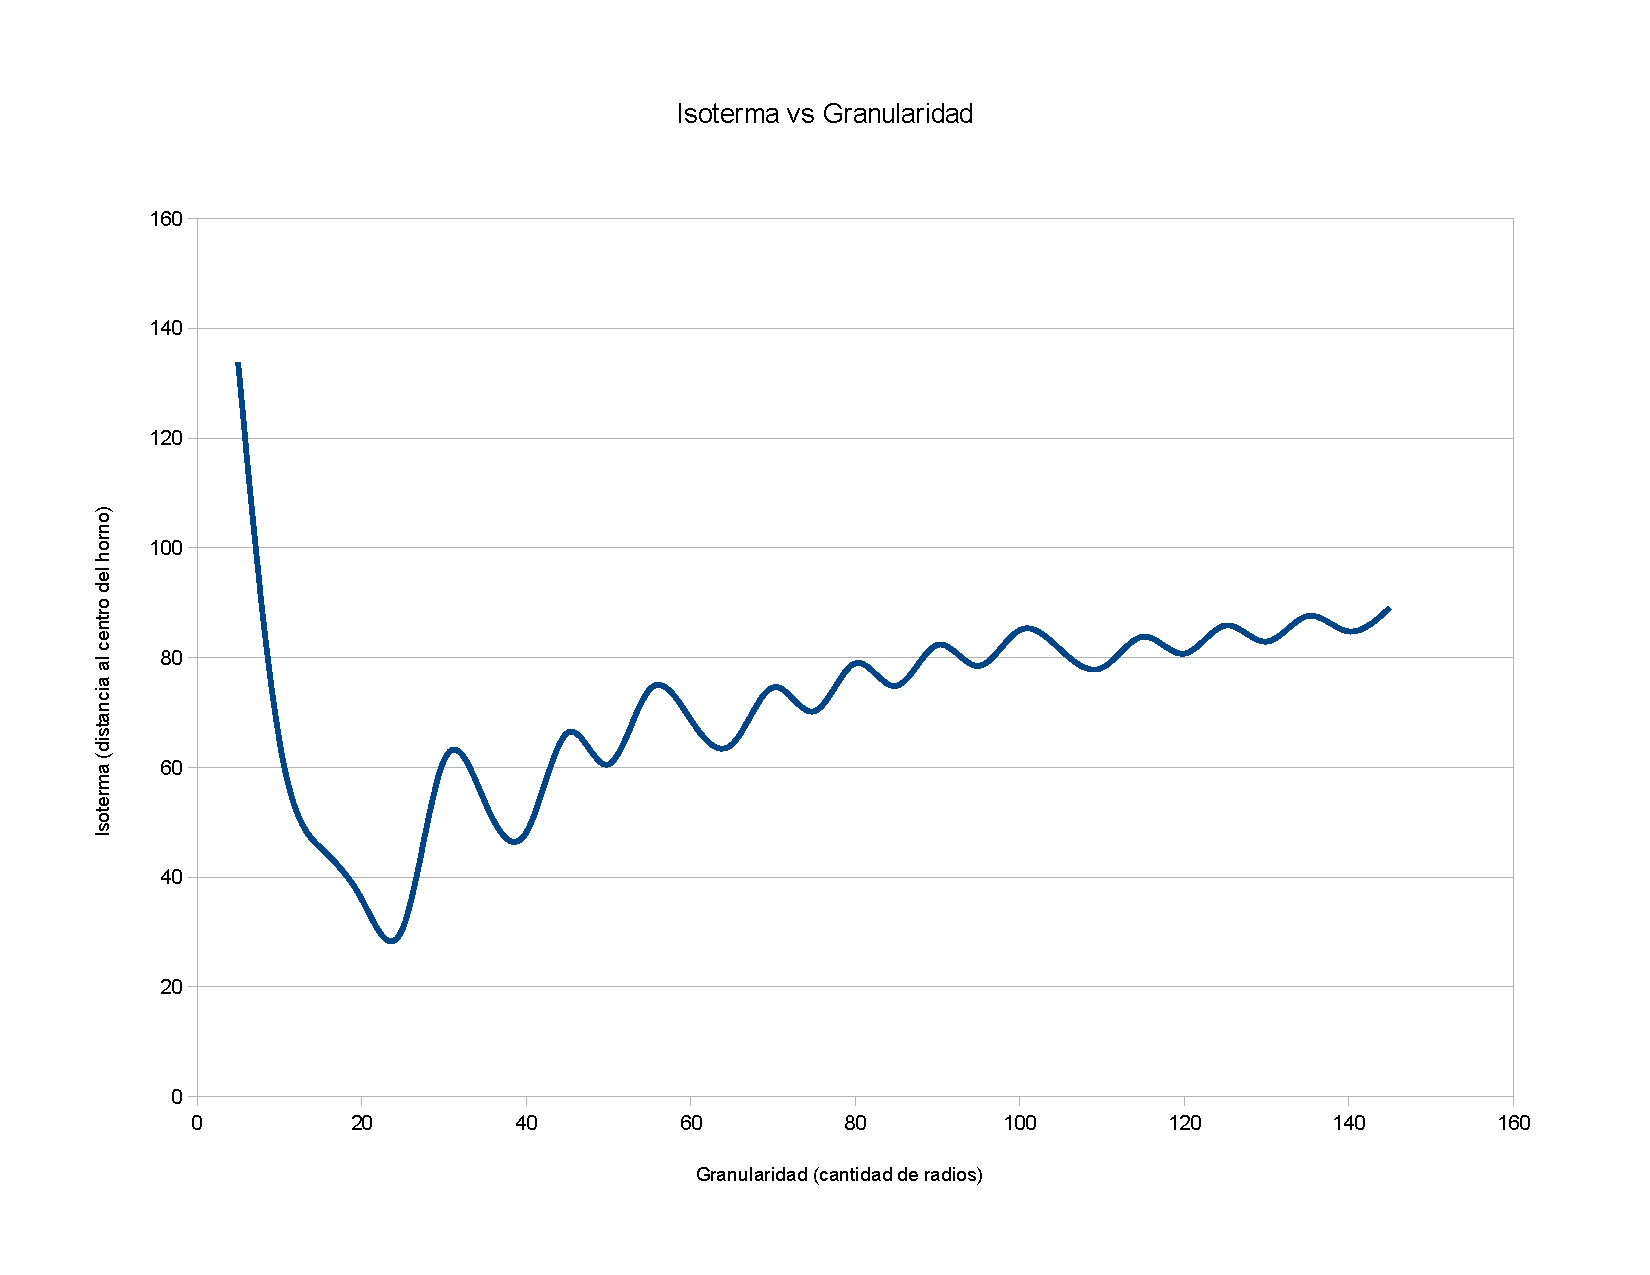
\includegraphics[scale=0.5]{graphs/IsotermaVsGranularidad.pdf}
\caption{Resulados obtenidos aumentando la cantidad de radios de 5 en 5.}
\label{isotermaVsGranularidad}
\end{figure}
A continuación mostramos los resultados obtenidos para el test de comparación entre factorización LU y eliminación gaussiana, los tiempos de cómputo se muestran en segundos y se usa escala logarítmica cuando es conveniente. Se muestran los resultados de matrices de 400x400, 225x225 y 100x100 


\begin{figure}[H]{}
\centering
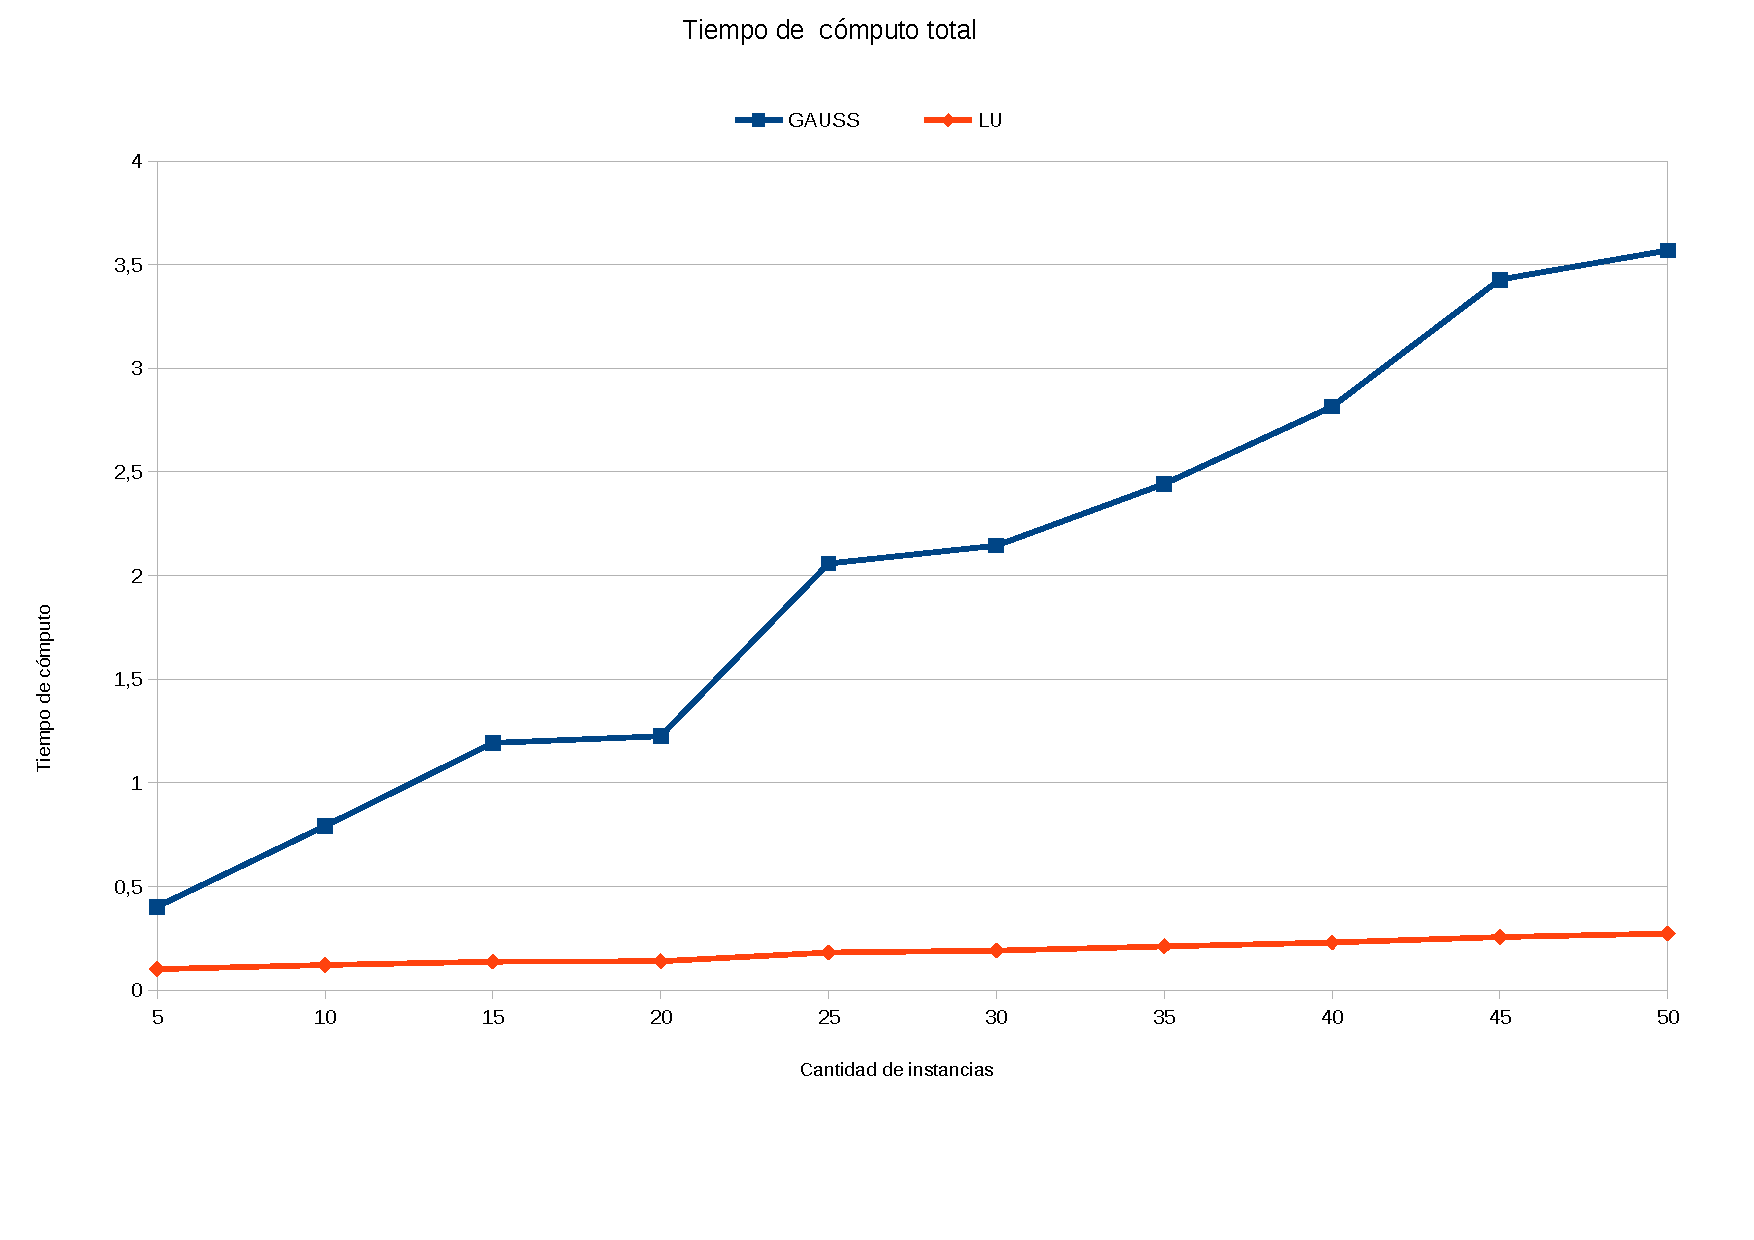
\includegraphics[scale=0.5]{graphs/gaussVsLU1.pdf}
\caption{Resultados obtenidos usando matrices de 20 ángulos y 20 radios. Se usa escala logarítmica.}
\label{gaussVsLU1}
\end{figure}

\begin{figure}[H]{}
\centering
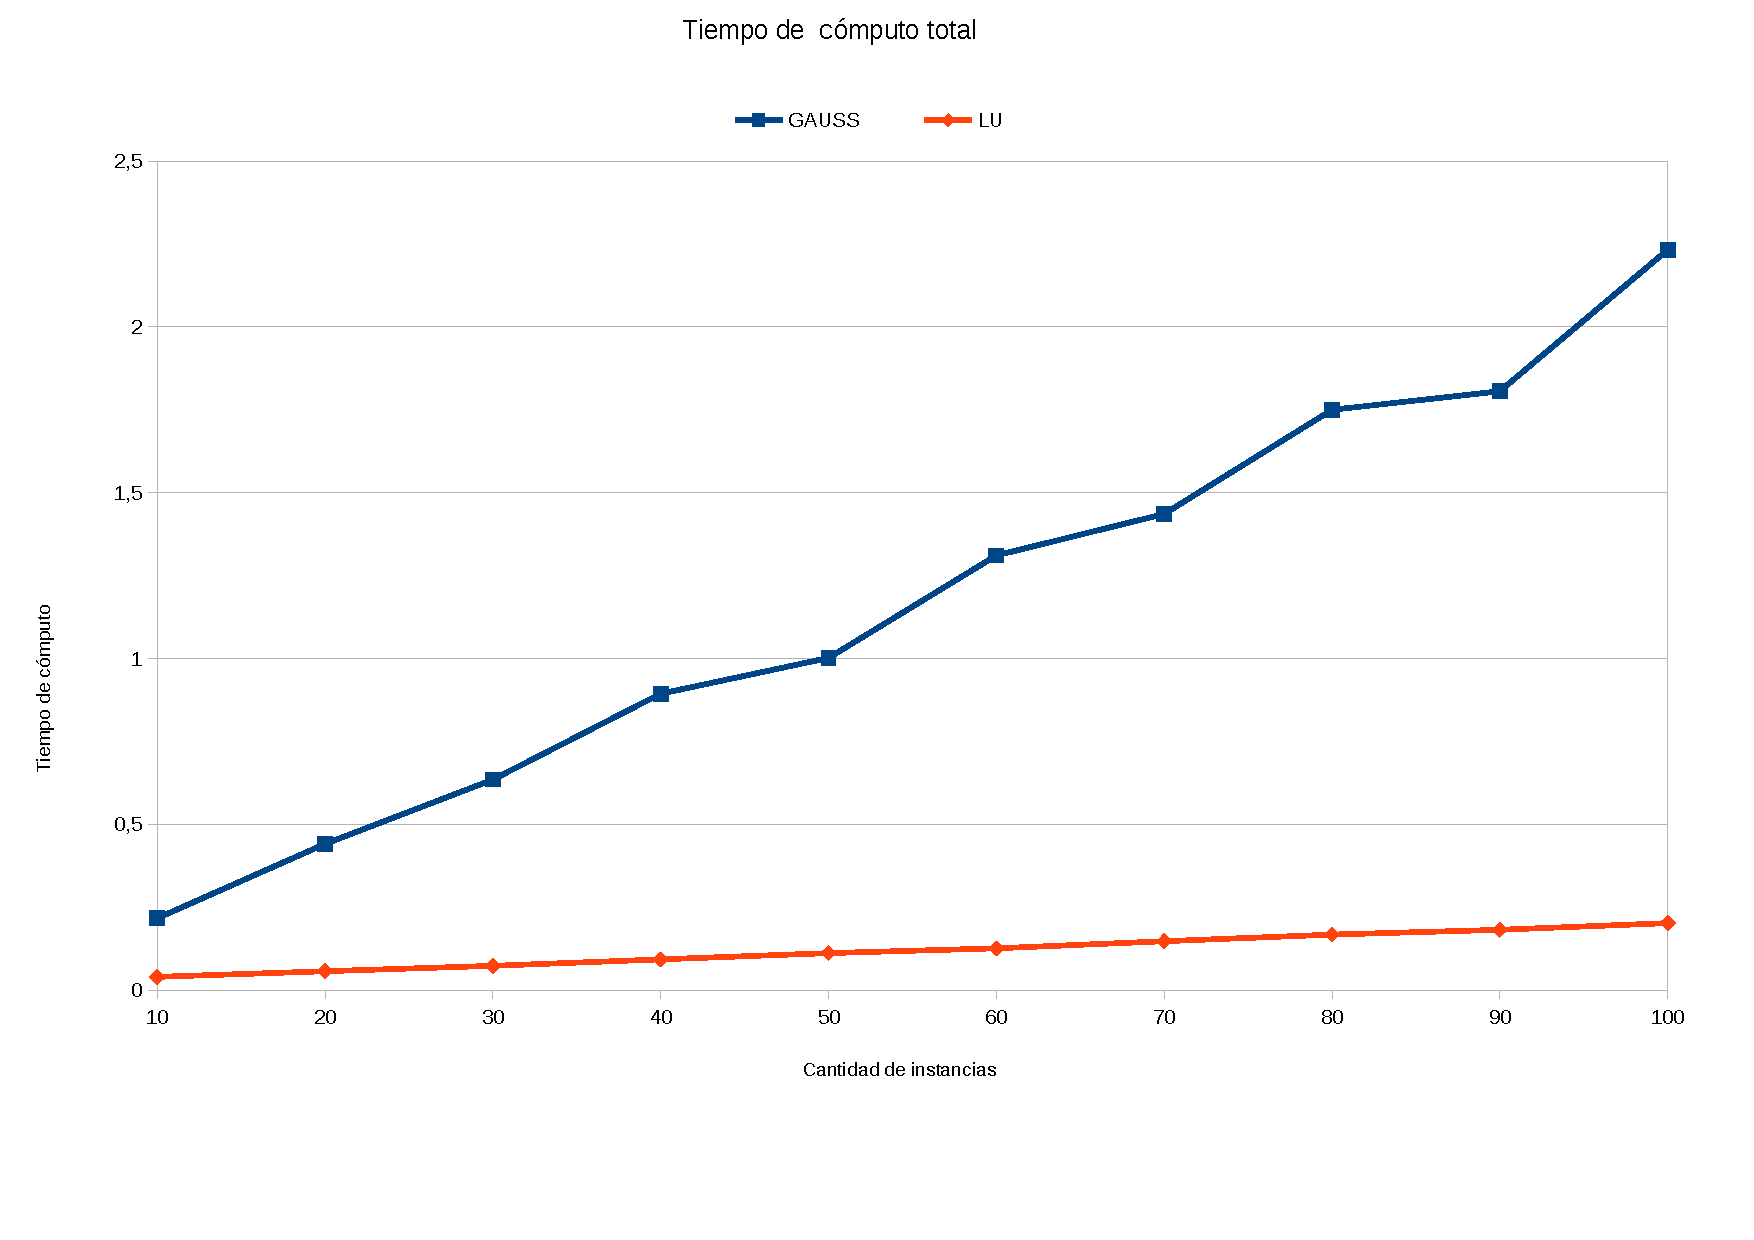
\includegraphics[scale=0.5]{graphs/gaussVsLU2.pdf}
\caption{Resultados obtenidos usando matrices de 15 ángulos y 15 radios. Se usa escala logarítmica.}
\label{gaussVsLU1}
\end{figure}

\begin{figure}[H]{}
\centering
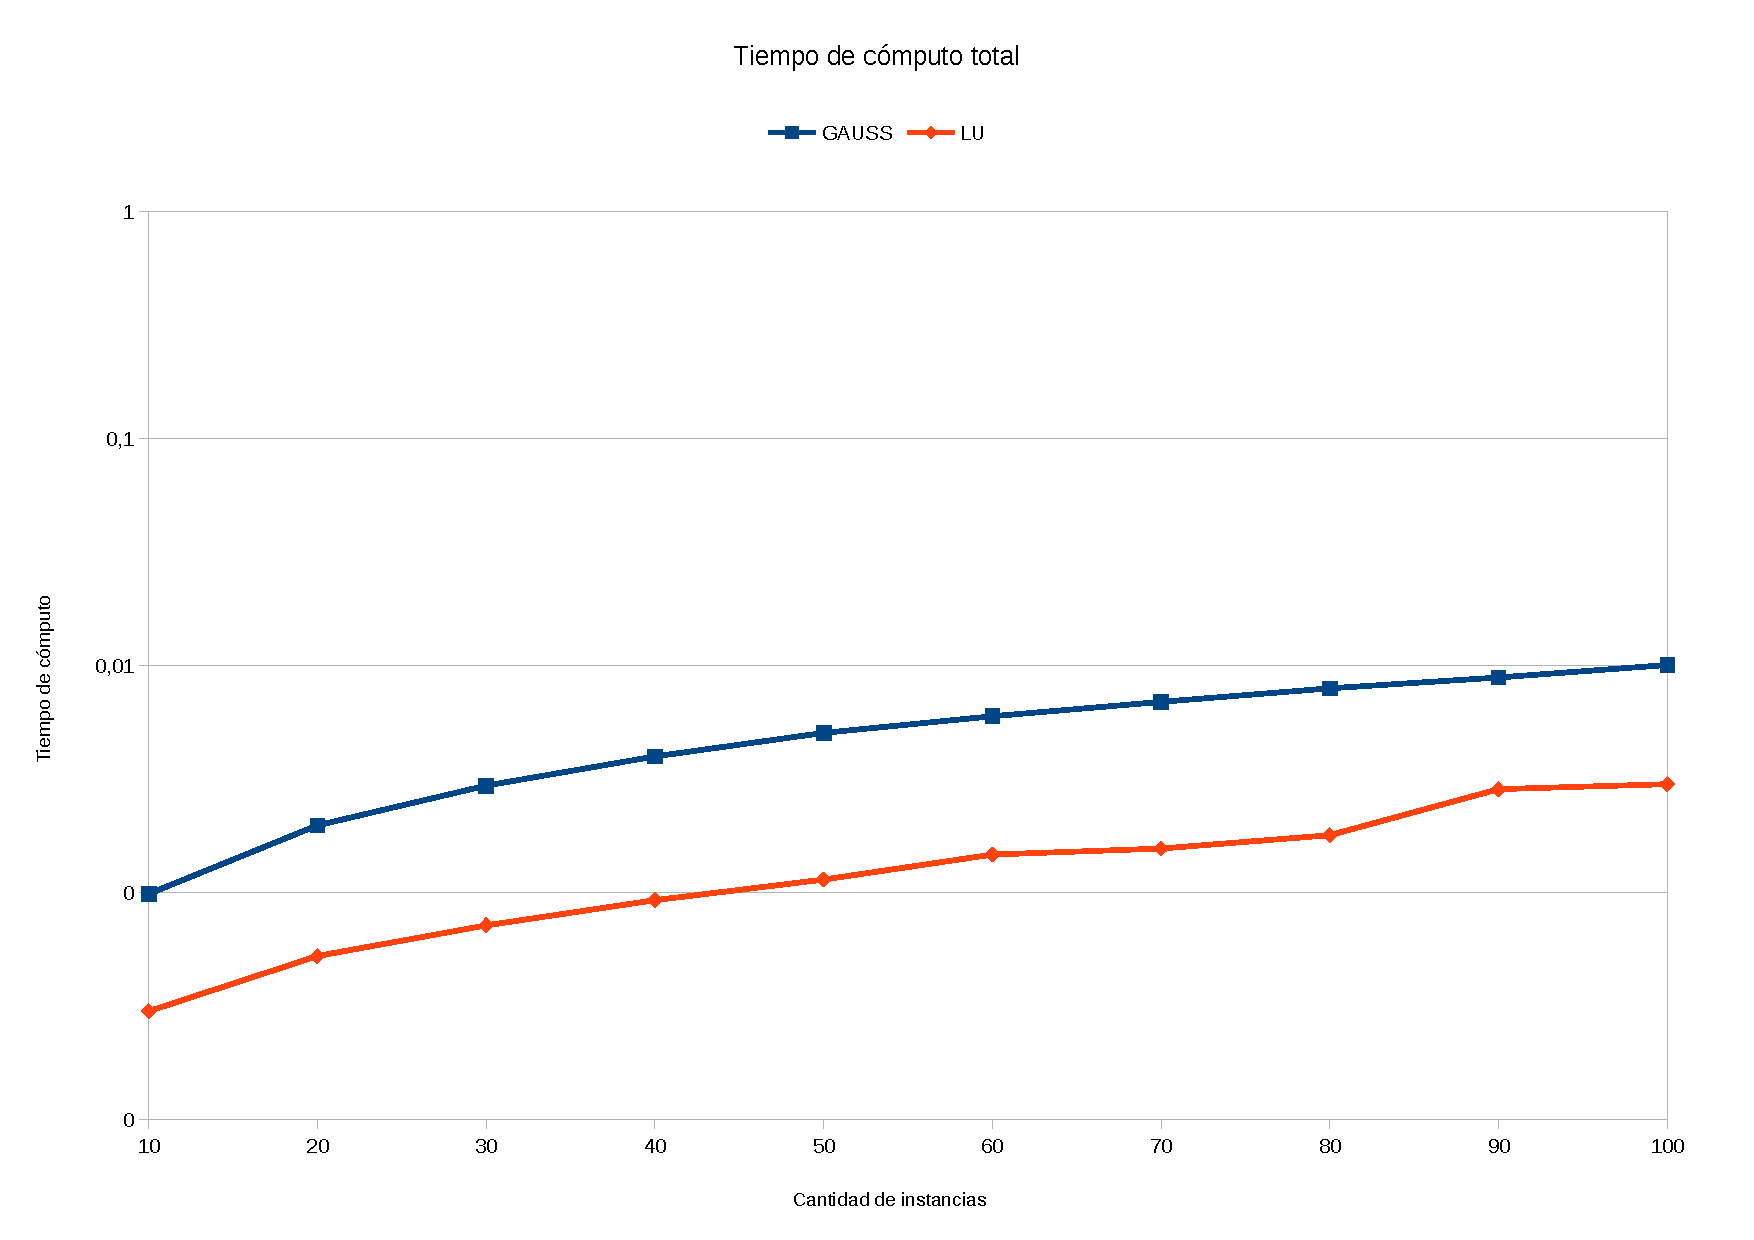
\includegraphics[scale=0.5]{graphs/gaussVsLU3.pdf}
\caption{Resultados obtenidos usando matrices de 10 ángulos y 10 radios. Se usa escala real.}
\label{gaussVsLU1}


\end{figure}

\subsection{Test de isoterma en función de las condiciones de borde}

La temperatura interna y externa aumentan a la misma velocidad. La isoterma buscada en todos los
casos es de $1500 ^{\circ}C$.

\begin{figure}[H]{}
\centering
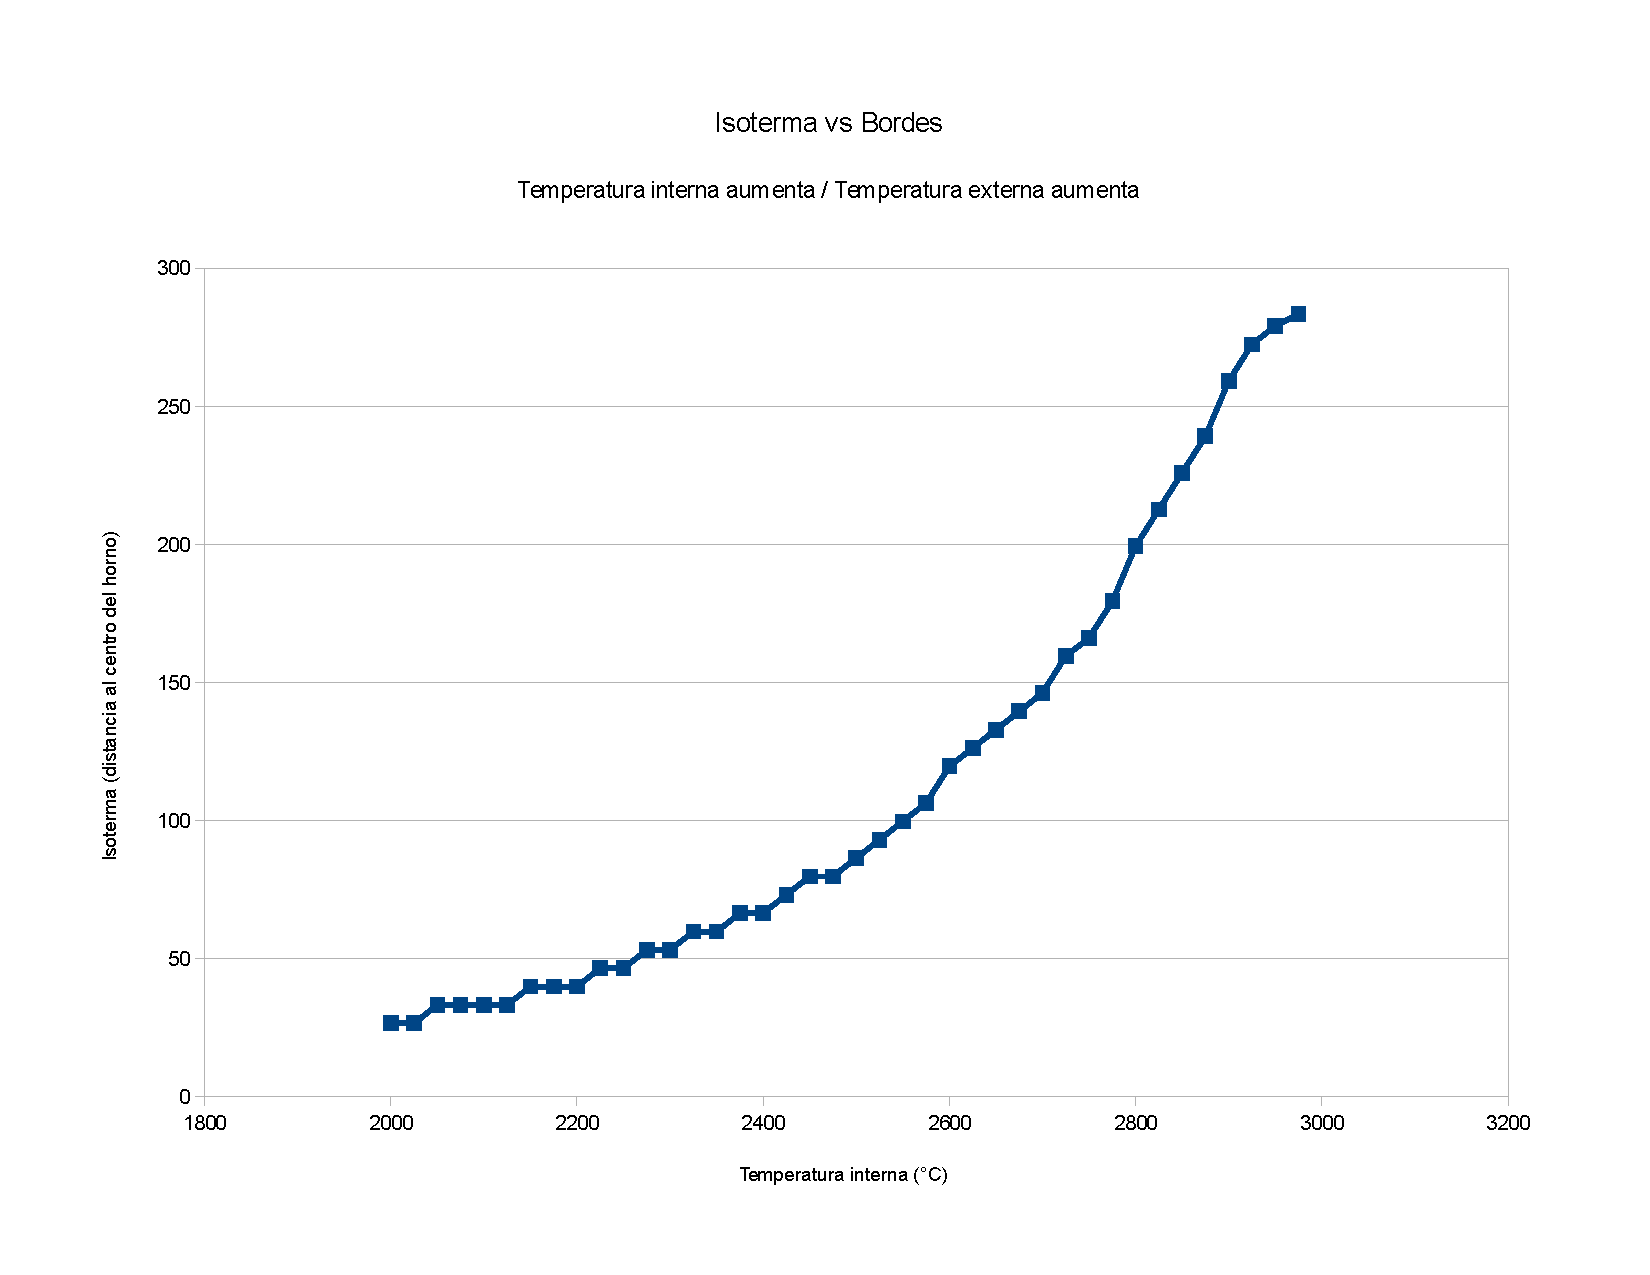
\includegraphics[scale=0.5]{graphs/isotermaVsBordesExternaAumenta.pdf}
\caption{La temperatura externa e interna a aumentan con la misma proporción. La temperatura externa empieza en 0 $^{\circ}C$}
\label{isotermaVsBordesExternaAumenta}
\end{figure}

\begin{figure}[H]{}
\centering
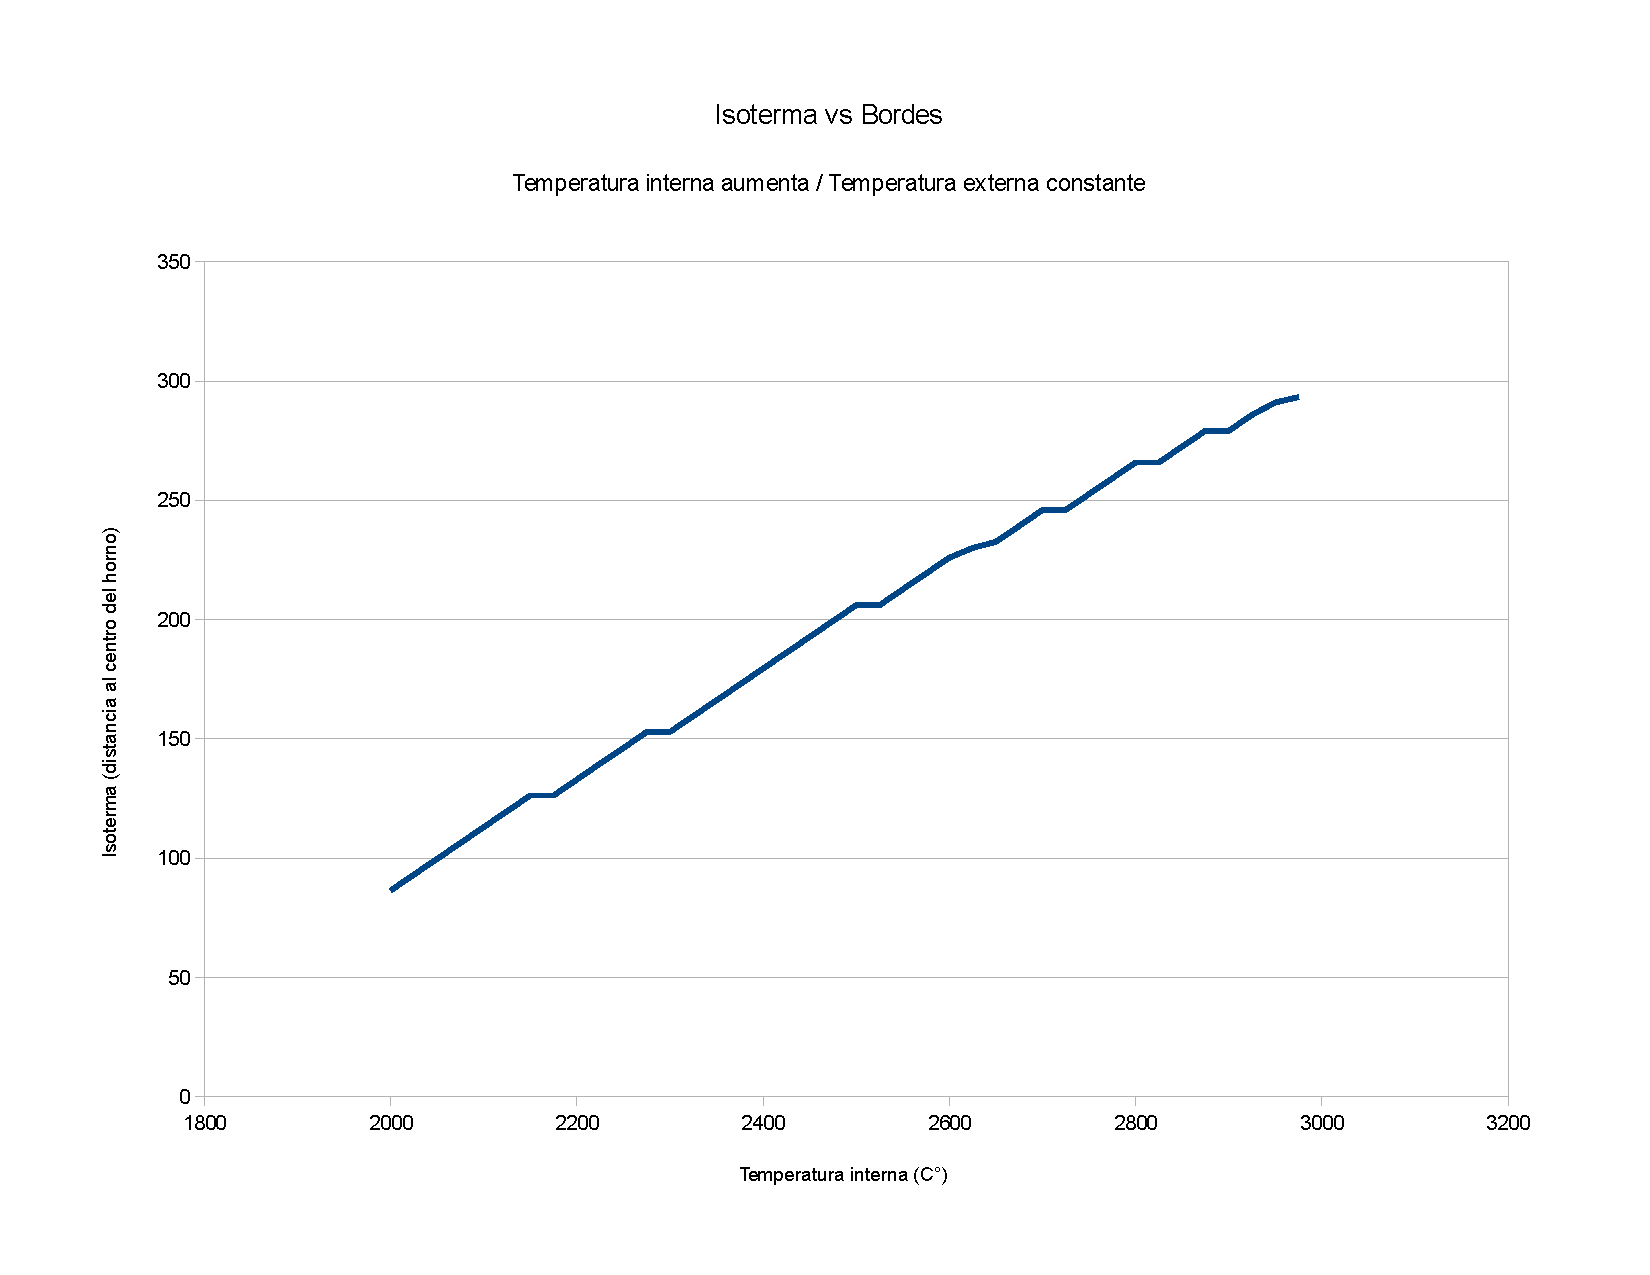
\includegraphics[scale=0.5]{graphs/isotermaVsBordesExternaConstante.pdf}
\caption{La temperatura externa se mantiene constante a 1000 $^{\circ} C$}
\label{isotermaVsBordesExternaConstante}
\end{figure}

La temperatura externa desciende a un $40\%$ la velocidad a la que aumenta la temperatura interna.

\begin{figure}[H]{}
\centering
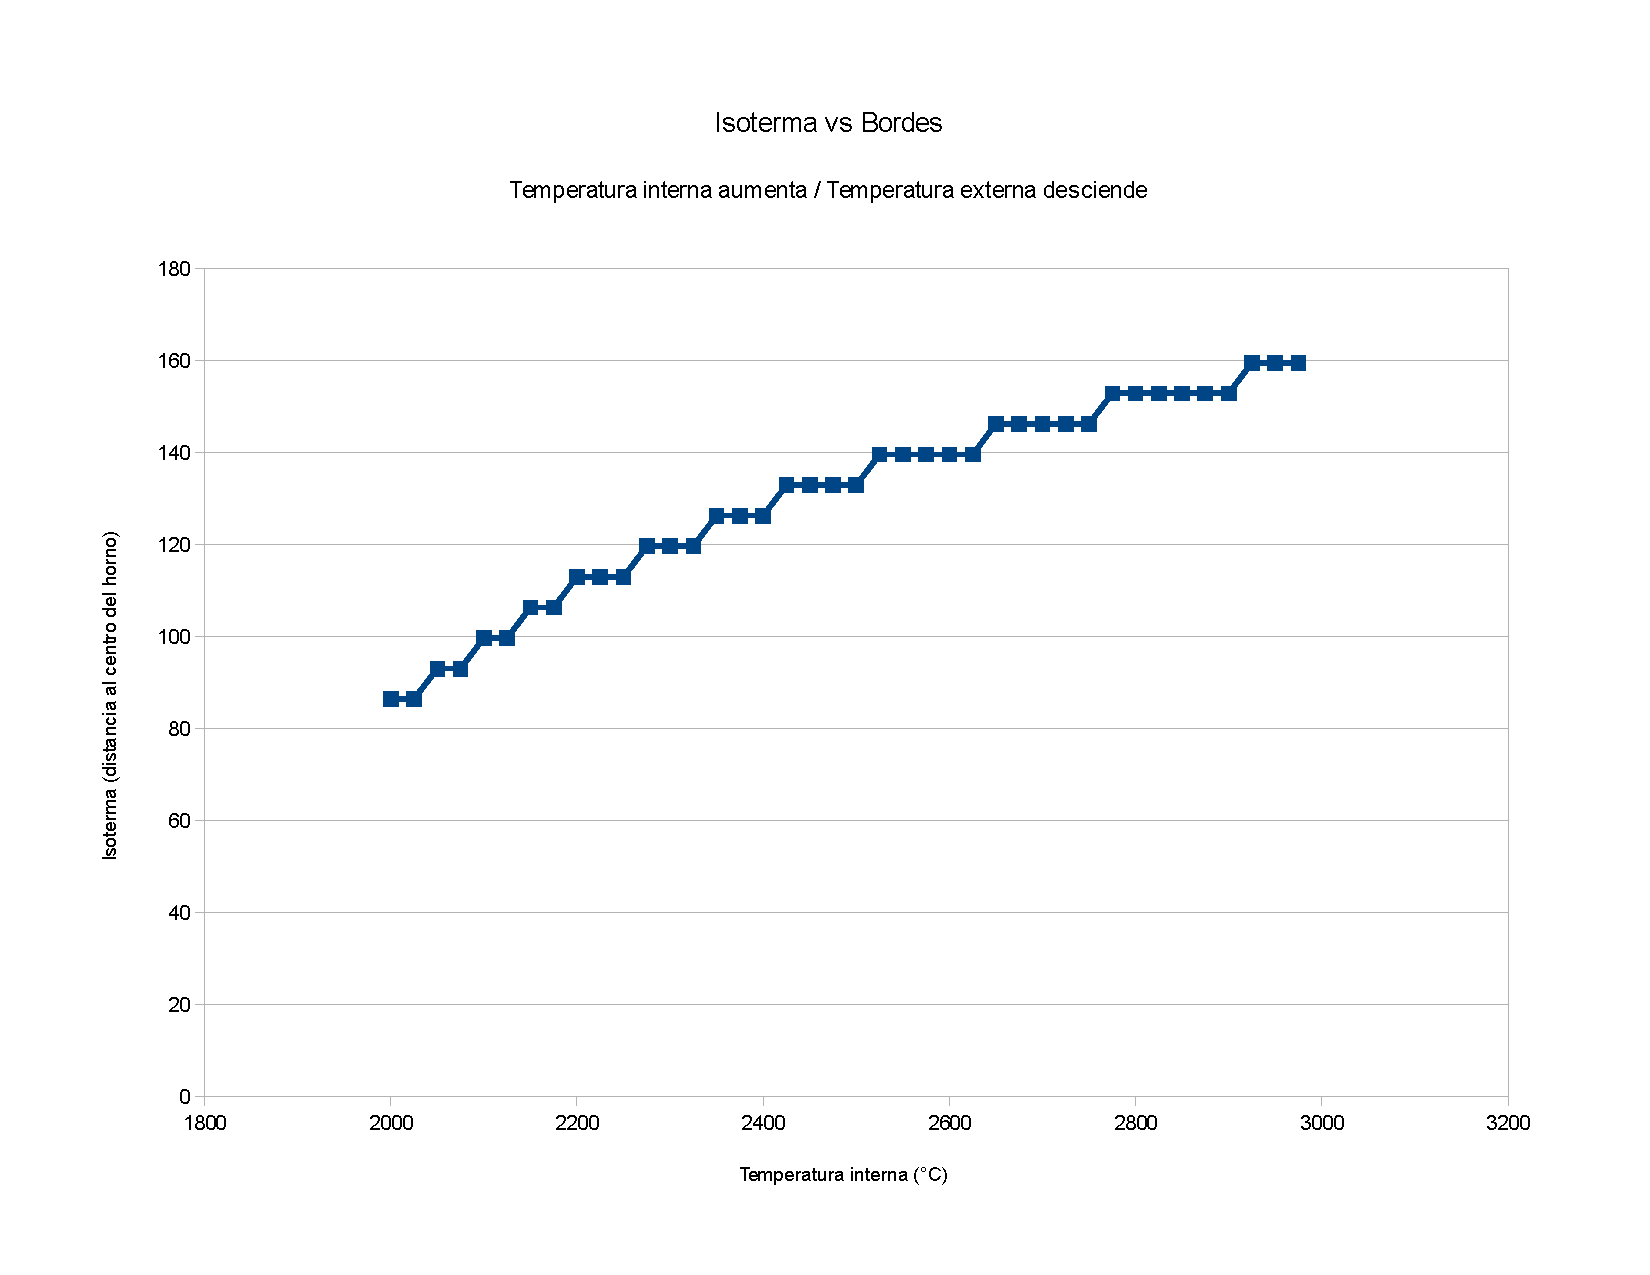
\includegraphics[scale=0.5]{graphs/isotermaVsBordesExternaDesciende.pdf}
\caption{La temperatura externa desciende más lento que lo que aumenta la interna.}
\label{isotermaVsBordesExternaDesciende}
\end{figure}

\subsection{Test de tiempo en función de la granularidad de la discretización}



\section{Discusión}
%Se incluirá aquí un análisis de los resultados obtenidos en la sección anterior (se analizará
%su validez, coherencia, etc.). Deben analizarse como míınimo los ítems pedidos en el
%enunciado. No es aceptable decir que “los resultados fueron los esperados”, sin hacer
%clara referencia a la teoría la cual se ajustan. Además, se deben mencionar los resul-
%tados interesantes y los casos “patológicos” encontrados.


\subsection{Análisis de comparación isoterma contra granularidad}
En el gráfico \ref{isotermaVsGranularidad} podemos ver claramente como en un principio aumentar un poco la granularidad 
nos cambia mucho el valor de la isoterma obtenida. Sin embargo, luego, a medida que la granularidad va en aumento, la 
isoterma va modificándose cada vez menos convergiendo a algún valor. Interpretamos que al aumentar la granularidad el 
valor obtenido para la isoterma converge a una magnitud, que corresponde a la isoterma real. Ésto coincide con la idea 
de que cuanta más precisión tengamos vamos a reducir el error de nuestros resultados. Creemos que la gran anomalía 
observada entre los primeros puntos del gráfico se debe a el reducido número de puntos utilizados en la 
discretización, esto provocaría un gran error en los resultados obtenidos con respecto al verdadero valor de la isoterma.
No sabemos certeramente a qué se debe la osilación presentada, sin embargo, creemos que simplemente se debe a cómo
se fue incrementando la discretización lo cual podría hacer que la isoterma se ubique de un lado u otro de el punto
de la discretización. Éste es un buen punto sobre el cual realizar otro experimento y contrastar los resultados.



\subsection{Análisis de comparación Gauss contra LU}
Como se puede apreciar en los gráficos \ref{gaussVsLU1}, \ref{gaussVsLU2} y \ref{gaussVsLU3}, al
variar la cantidad de instancias el tiempo de cómputo de la factorización LU fue muy inferior al
tiempo de la eliminación gaussiana, y esta diferencia se hace sumamente notoria a medida que la
cantidad de vectores $b$ (a partir de ahora simplemente ``instancias'') a calcular aumenta. En el gráfico 
\ref{gaussVsLU4} se puede observar como la diferencia es proporcional tanto a la cantidad de instancias como al 
tamaño de las matrices, es decir, al aumentar la cantidad de instancias y/o el tamaño de la matriz LU aumenta 
la diferencia con respecto a Gauss. Por otro lado en \ref{gaussVsLU5} se puede determinar que basta con resolver el 
sistema de ecuacionescon sólo dos vectores $b$ distintos para poder ya apreciar una ventaja efectiva sobre la eliminación gaussiana 
y que para el caso en que solo haya un sólo vector $b$, los tiempos de cómputo son prácticamente idénticos, es decir la 
\emph{forward substitution} extra no agrega \emph{overhead} al cálculo de la solución. También es posible notar que para 
los diferentes tamaños matriciales, la relación se mantiene para una misma cantidad de instancias, y que dicha relación 
muestra una incremento significativo a medida que se se incrementa la cantidad de instancias, por lo que se puede determinar 
que el factor más importante que influye sobre la diferencia de rendimiento entre eliminación gaussiana es la cantidad de 
instancias y no tanto el tamaño de la matriz.

\subsection{Análisis de comparación isoterma en función de las condiciones de borde}

El gráfico \ref{isotermaVsBordesExternaAumenta} muestra claramente que al aumentar la temperatura
externa e interna en la misma proporción la isoterma se mueve cada vez más rápido hacia el borde que
se acerca a ella. En este caso es el borde externo. La temperatura externa empieza en 0 $^{\circ}C$ y
finaliza en 1000 $^{\circ}C$. Esto coincide con lo que esperaríamos en una situación real.  En el gráfico
\ref{isotermaVsBordesExternaConstante} mantuvimos la temperatura externa constante por lo tanto la
isoterma siguió acercándose al borde exterior pero siempre al mismo ritmo. Interpretamos que se
acerca con velocidad lineal porque es la velocidad a la que crece la temperatura interna.
Finalmente, en el gráfico \ref{isotermaVsBordesExternaDesciende} vemos claramente cómo el movimiento
de los bordes va afectando directamente a la posición de la isoterma y en sus mismas proporciones. A
pesar de que la temperatura externa desciende mientras que la interna asciende, la isoterma sigue
acercándose hacia el borde externo. Ésto se debe a que la temperatura externa desciende a un $40\%$
la velocidad a la que aumenta la interna.  Después de analizar éstos tres gráficos concluimos que el
modelo implementado coincide en gran parte con lo que el sentido común indica. El valor de la
isoterma va modificándose de forma directamente proporcional a el cambio de las temperaturas
internas y externas que ejercen influencia sobre ella en sentidos contrarios.

\subsection{Análisis de comparación de granularidad y tiempo}
Como era de esperarse, el tiempo de ejecución es creciente con la granularidad y, además,
aparentaría ser cúbico con una función con multiplicadores extraños. Esto no debería ser de
demasiada sorpresa dado que estamos midiendo en segundos y el tiempo es siempre menor a 15 segundos.
Si tenemos en cuenta esto y además que la granularidad va desde $30^2$ hasta $100^2$, no parece tan
alocado tener que dividir por $10^{11}$ y multiplicar por 2.

Éste fue un test satisfactorio dado que ocurrió lo que esperábamos: poder acotar el crecimiento de
los tiempos por una función cúbica y sin resultados extraños inesperados. Sí hay algunas pequeñas
irregularidades en los puntos, pero, aunque incomprobable, bien podría ser responsabilidad del
scheduler del sistema operativo u otra de todas las variables que podrían haber afectado mínimamente
los resultados, aún sacando promedio en 5 instancias.

% % Lo que sí
% descubrimos en este test es que el tiempo parece crecer más que linealmente dado que la pendiente
% de la función que parecerían describir los datos es mayor que la de la función lineal que usamos
% para comparar. Esto en un principio parecería intuitivo dado que la complejidad de nuestros
% algoritmos depende de la matriz A en la ecuación Ax=b, y las dimensiones de ésta dependen de la
% granularidad, pero de la granularidad al cuadrado. Por ende, mientras más crece la granularidad más
% crece la dimensión de la matriz, pero cuadráticamente.



\section{Conclusiones}
%Esta sección debe contener las conclusiones generales del trabajo. Se deben mencionar
%las relaciones de la discusión sobre las que se tiene certeza, junto con comentarios
%y observaciones generales aplicables a todo el proceso. Mencionar también posibles
%extensiones a los métodos, experimentos que hayan quedado pendientes, etc.
Como ya se mencionó, este trabajo tiene dos secciones principales: una es la resolución se sistema de 
ecuaciones lineales mediante técnicas algorítmicas matriciales, y la otra es el problema de estimar una 
isoterma a partir de una cantidad finita de puntos con sus correspondientes temperaturas. Para la parte 
inicial se estudió la eliminación gaussiana y la factorización LU. Pese a que son muy 
parecidas en su defición y en su implementación algorítmica, es preferible usar la segunda en caso
de que se necesite resolver un sistema para una misma matriz $A$, pero distintos vectores $b$ 
ya que reduce el costo computacional de manera contundente. 

Una desventaja es que la factorización LU no siempre existe. Sin embargo, siempre que exista es
preferible utilizarla antes que la eliminación gaussiana clásica. Más aun, cuanto más vectores 
b distintos haya, mayor será diferencia entre ambos algoritmos. Cabe señalar que la factorización LU no 
requiere espacio de memoria adicional ni agrega complejidad al algoritmo de eliminación gaussiana sin pivoteo.

En el caso de los tests con la isoterma, nuestros algoritmos se acercaron a lo que se esperaría de
la realidad, o la realidad se acercó a lo que se esperaba de nuestros algoritmos, cómo se quiera
verlo. Mientras más ricos seamos en la industria del tiempo de cómputo, más granularidad podremos
permitirnos comprar, y más exacta será nuestra isoterma.

También fue el caso que la isoterma tendía a acercarse a la pared que más debía acercarse según
nuestras predicciones, confirmando empíricamente que nuestras acepciones sobre las leyes físicas y
nuestro entendimiento de la fórmula de expansión del calor eran correctas.

Como trabajo práctico en general, fue una experiencia nueva. Aprendimos a prestarle más atención al
por qué hacíamos las cosas en vez de cómo hacerlas.






\section{Apéndices}
\subsubsection{Demostración de la proposición}
Proposición:

Sea $A \in K^{n \times n}$ con $K$ $=$ $\mathbb{R}$ o $\mathbb{C}$ una matriz diagonal dominante e inversible entonces es posible aplicar eliminación gaussiana sin pivoteo.

Notación útil: 

$A(i|j)$ := Es la submatriz de $A$ que se obtiene de elimar las filas de $1$ a $i$ y las columnas de $1$ a $j$.

$A^{(k)}$ := Es la matriz obtenida luego de relizar $k$ pasos de eliminación gaussiana sobre las filas de $A$.

Demostración:

Como A es diagonal dominante, se tiene que $|A_{ii}|$ $\geq$ $\sum_{j=1, i \neq j}^{n}$ $|A_{ij}|$ para todo $j$ $\neq$ $i$, por lo tanto debe suceder que $A_{11}$ $\neq$ $0$, si así no fuera, se tiene que $0$ $=$ $|A_{11}|$ $\geq$ $|A_{1j}|$  $\geq$ $0$ para todo $j$ $\neq$ $2$ a $n$, por lo que $|A_{1j}|$ $=$ $0$, y esto sucede si y solo si $A_{ij}$ $=$ $0$, es decir, la columna $1$ es nula y por lo tanto A no es inversible, pero A es inversible y en consecuencia $A_{11}$ $\neq$ $0$.
Teniendo en cuenta que $A_{11}$ $\neq$ $0$, veamos ahora que al realizar eliminación gaussiana sobre $A$, la matriz $A(1|1)^{(1)}$ resulta ser diagonal dominante:
Hay que probar que para todo $j$ vale:
\[
\sum_{i \geq 2, i \neq j}^{n}|A_{ij}^{(1)}| \leq  |A_{jj}^{(1)}| 
\]
Tenemos que:
\[
\sum_{i \geq 2, i \neq j}^{n} |A_{ij}^{(1)}| =  \sum_{i \geq 2, i \neq j}^{n} |A_{ij} - \frac{A_{1j}A_{i1}}{A_{11}}| \leq 
\sum_{i \geq 2, i \neq j}^{n} |A_{ij}| + |\frac{A_{1j}A_{i1}}{A_{11}}| =
\sum_{i \geq 1, i \neq j}^{n} |A_{ij}| - |A_{1j}| + |\frac{A_{1j}}{A_{11}}|(\sum_{i \geq 2}^{n} |A_{i1}| - |A_{j1}|)
\]
y como A es diagonal dominante:
\[
\sum_{i \geq 1, i \neq j}^{n} |A_{ij}| \leq |A_{jj}| \text{\qquad y \qquad} \sum_{i \geq 2}^{n} |A_{i1}| \leq |A_{11}
\]
Finalmente:
\[
\sum_{i \geq 1, i \neq j}^{n} |A_{ij}| - |A_{1j}| + |\frac{A_{1j}}{A_{11}}|(\sum_{i \geq 2}^{n} |A_{i1}| - |A_{j1}|) \leq
|A_{jj}| - |A_{1j}| + |\frac{A_{1j}}{A_{11}}|(|A_{11} - |A_{j1}|) =
\]

\[
|A_{jj}| - |\frac{A_{1j}A_{j1}}{A_{11}}| \leq
|A_{jj} - \frac{A_{1j}A_{j1}}{A_{11}}| = |A_{jj}^{(1)}|
\]

Por lo tanto $A(1|1)^{(1)}$ es diagonal dominante, y volviendo a utilizar la demostración anterior en cada paso de la eliminación gaussina se concluye que A es diagonalizable sin pivoteo.


%En el apéndice A se incluirá el enunciado del TP. En el apéndice B se incluirán los
%códigos fuente de las funciones relevantes desde el punto de vista numérico. Resultados
%que valga la pena mencionar en el trabajo pero que sean demasiado específicos para
%aparecer en el cuerpo principal del trabajo podrán mencionarse en sucesivos apéndices
%rotulados con las letras mayusculas del alfabeto romano. Por ejemplo: la demostración
%de una propiedad que aplican para optimizar el algoritmo que programaron para resolver
%un problema.



%\section{Referencias}
%Es importante incluir referencias a libros, artículos y páginas de Internet consultados
%durante el desarrollo del trabajo, haciendo referencia a estos materiales a lo largo del
%informe. Se deben citar también las comunicaciones personales con otros grupos.
\addcontentsline{toc}{section}{Referencias}
\begin{thebibliography}{1}
\bibitem{burden} Richard Burden. \textbf{Numerical Analysis.}  Brooks Cole, 2000.
\end{thebibliography}


\newpage
\bibliographystyle{plain}


\end{document}
